\begin{document}

\newcommand{\TODO}[1]{\todo[inline,color=red!20]{#1}}

\title{Cloudmesh in support of the\\NIST Big Data Architecture Framework}


\numberofauthors{2} 
\author{
\alignauthor
Gregor von Laszewski, Badi Abdul-Wahid, Fugang Wang, Hyungro Lee, Geoffrey C. Fox\\
       \affaddr{Indiana University}\\
       \affaddr{Bloomington, IN}\\
       \email{laszewski@gmail.com}
\alignauthor
Wo Chang\\
       \affaddr{NIST Big Data Public Working Group}\\
       \affaddr{National Institute of Standards and Technology}\\
       \email{wo.chang@nist.gov}
}
\date{20 April 2013}

\maketitle



\begin{abstract}

  The National Institute of Standards and Technology (NIST) has
  provided a big data reference architecture and is currently
  attempting to validate that architecture. As part of our current
  efforts we have developed cloudmesh client a tool that sets its goal
  towards easily managing clouds, container, batch queues and bare
  metal infrastructure. It also allows the integration of defined
  software stacks that can be used to deploy complex and
  state-of-the-art frameworks with devOps tools. Cloudmesh is on
  purpose designed to be vendor agnostic. We evaluate in this paper
  two aspects. First, based on our rich experience with clouds and
  other infrastructures, {\it can we verify the NIST reference
    architecture from our point of view?} Second, {\it which
    limitations may exist in cloudmesh client that need to be
    addressed to potentially improve integration with the NIST
    efforts?}  We will see in this paper that cloudmesh validates the
  NIST big data architecture which itself motivated further
  improvements to cloudmesh that we have implemented.
\end{abstract}


\section{Introduction}

Commercial, academic, and government leaders agree about the potential
of {\em} Big Data to spark innovation, fuel commerce, and drive
progress. Big Data is the common term used to describe the deluge of
data in today’s networked, digitized, sensor-laden, and information
driven world \cite{nist-bd}. Desirable is as a vendor neutral,
technology- and infrastructure-agnostic conceptual model and examine
related issues.  The focus of this document is on the Big Data
Application Reference Archoitecture and identify lessons learned from
cloudmesh that can augment and verify this architecture through
practical use cases. In the next sections we provide some background
information to motivate our work and to introduce the two frameworks
motivating this paper. This includes cloudmesh \cite{las12-cloud}
\cite{github-cloudmesh-client} and the NIST big data reference
architecture \cite{nist-bd}.  We start by giving brief introductions
to the National Institute of Standards (NIST) big data reference
architecture (Section \ref{S:NBDarch}) followed by a brief
introduction to Cloudmesh (Section \ref{S:cmclient}).  We then
\TODO{describe the next sections}

\subsection{NBD Reference Architecture}
\label{S:NBDarch}

The NIST big data working group is exploring pathways
forward in this direction which can be leveraged by the community. The
current result reference architecture is summarized in
\cite{nist-bd}. From this document we gather that the {\it
  ``conceptual model, referred to as the NIST Big Data Reference
  Architecture (NBDRA), was crafted by examining publicly available
  Big Data architectures representing various approaches and
  products. Inputs from the other NBD-PWG subgroups were also
  incorporated into the creation of the NBDRA. It is applicable to a
  variety of business environments, including tightly integrated
  enterprise systems, as well as loosely coupled vertical industries
  that rely on cooperation among independent stakeholders. The NBDRA
  captures the two known Big Data economic value chains: information,
  where value is created by data collection, integration, analysis,
  and applying the results to data-driven services, and the
  information technology (IT), where value is created by providing
  networking, infrastructure, platforms, and tools in support of
  vertical data-based applications.''}  It will produce a number of
documents related to definitions \cite{??}, taxonomies \cite{??}, use
cases and general requirements \cite{??}, security and privacy
\cite{??}, architectures white paper survey \cite{??}, reference
architecture \cite{??}, standards roadmap \cite{??}, and an interface
definition \cite{??}.

\TODO{Hyungro: add citations to the NIST documents related to this}

One of the desired tasks is to identify existing frameworks and to
analyze how they correlate to the current reference architecture
\cite{nist-bd}. This is conducted in order to validate and if needed
to improve the architecture.  The current NIST big data reference
architecture is shown in Figure~\ref{F:NIST-arch}. However we have
augmented the architecture with areas where cloudmesh interfaces with
it. We will describe the offerings in relationship to this
architecture of cloudmesh in detail in Section \ref{S:cm-nist}.  The
NIST BDA contains according to \cite{nist-bd} the following
components and services:

\TODO{find uniform abbreviation}

\TODO{define a cm nist section}

\begin{figure}[hp]
  \centering
     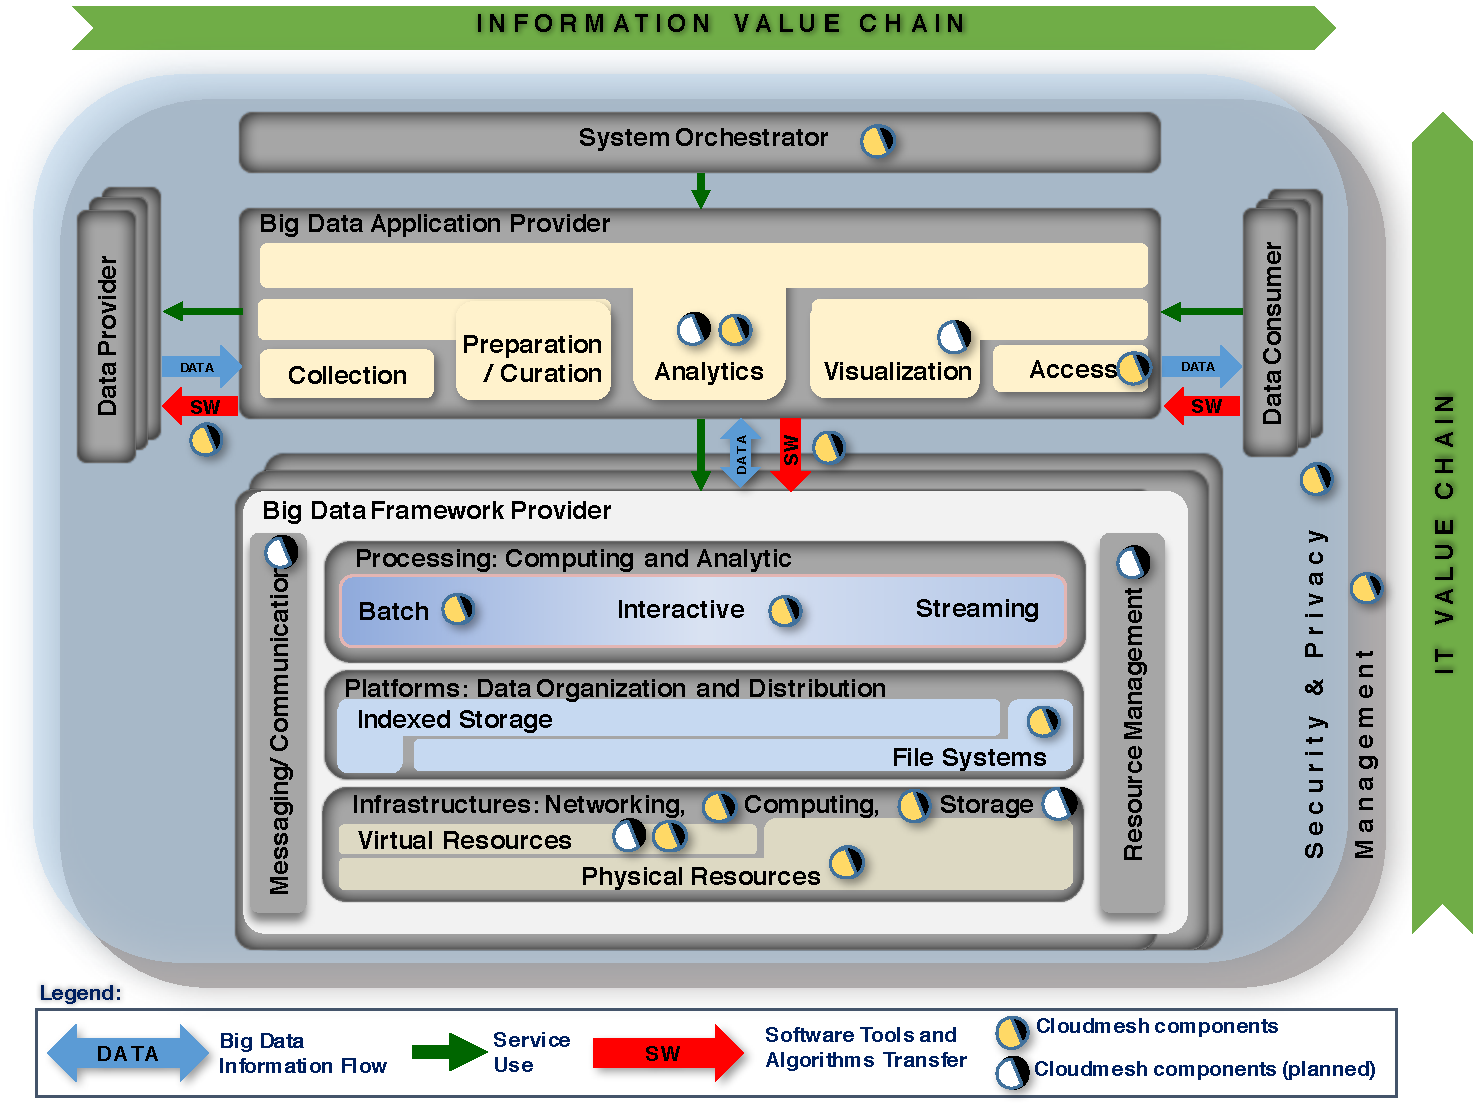
\includegraphics[width=1.0\columnwidth]{images/nist-bda.pdf}
  \caption{NIST Big Data Reference Architecture (NBDRA) diagram} 
  \label{F:NIST-arch}
%\end{figure}

\bigskip
%\begin{figure}[htb]
  \centering
     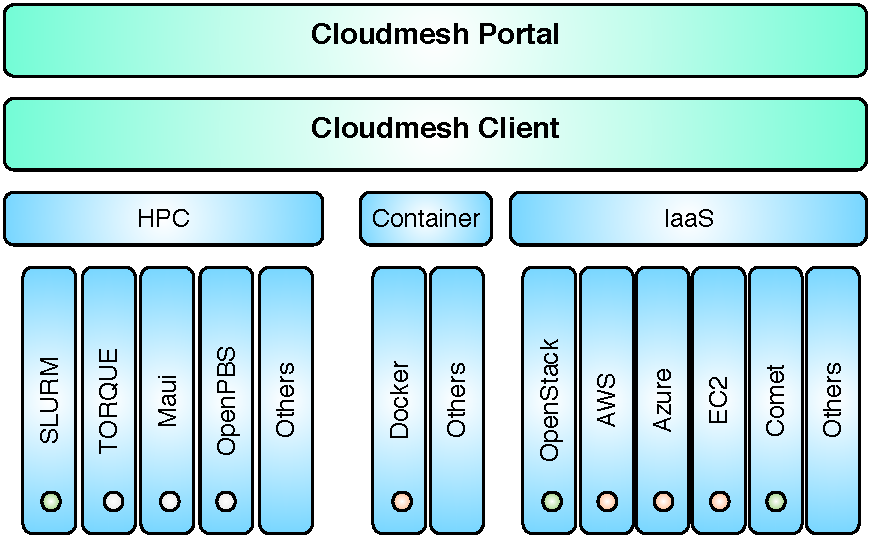
\includegraphics[width=1.0\columnwidth]{images/cloudmesh-arch-1.pdf}
  \caption{Cloudmesh layered architecture.} 
  \label{F:NIST-arch}
%\end{figure}
\bigskip

%\begin{figure}[htb]
  \centering
      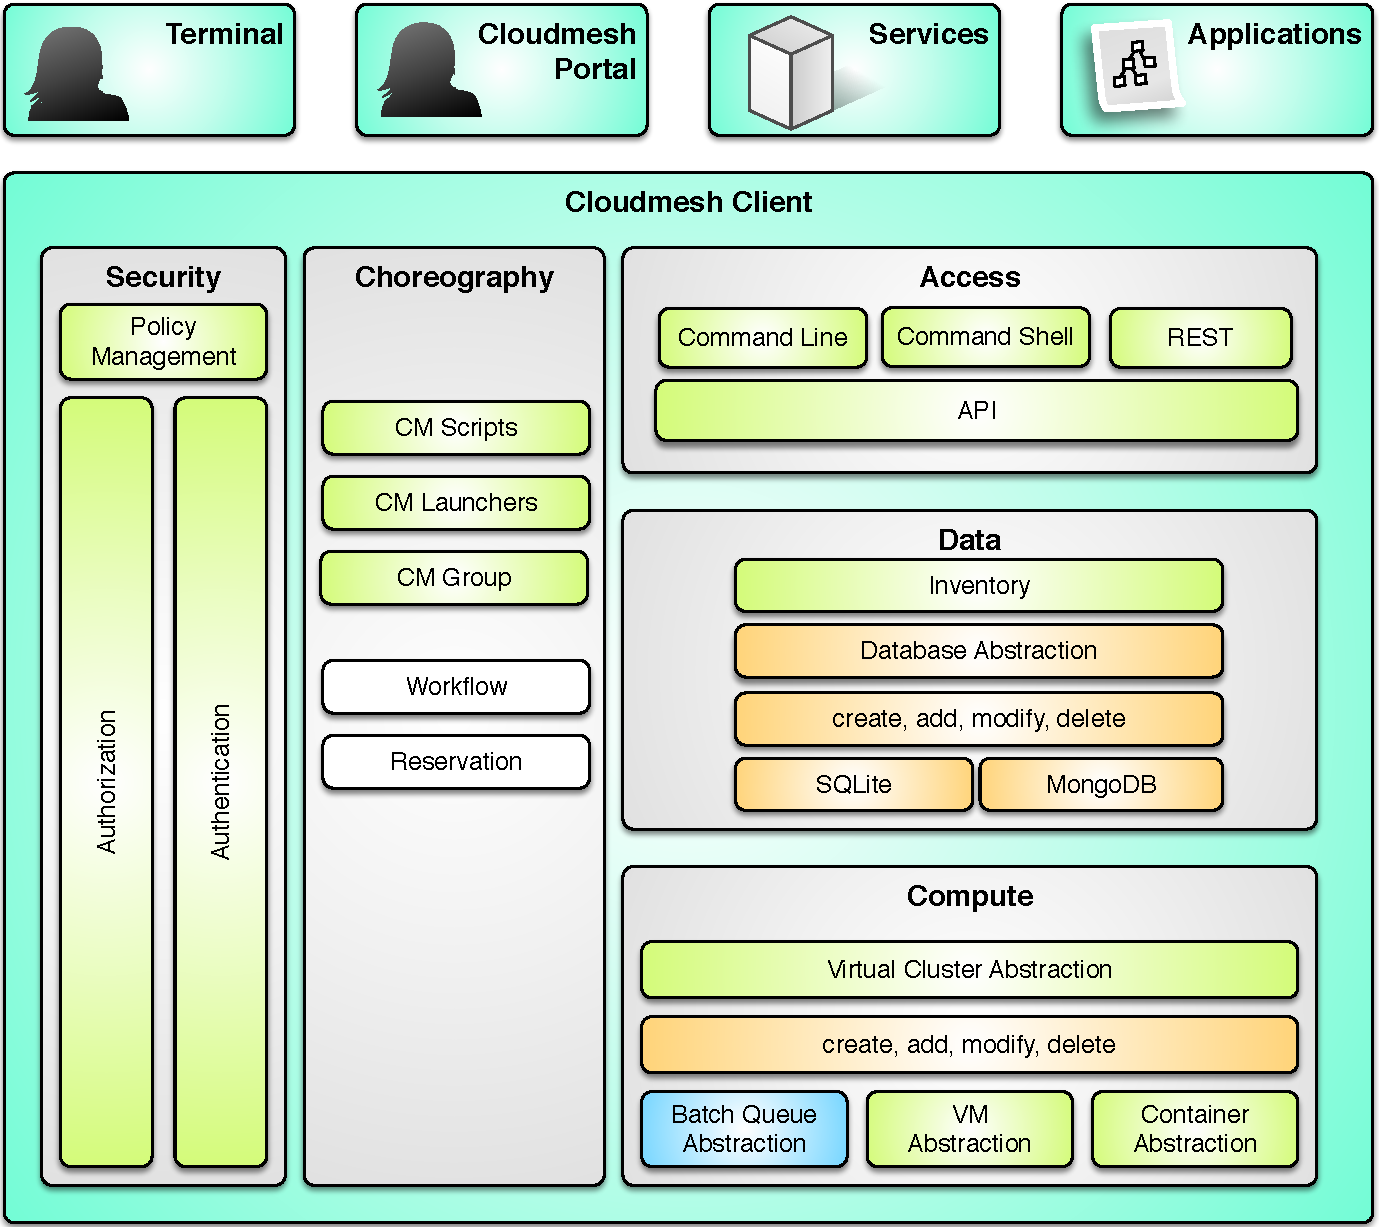
\includegraphics[width=1.0\columnwidth]{images/cloudmesh-arch-2.pdf}
  \caption{Cloudmesh components.} 
  \label{F:NIST-arch}
\end{figure}

\begin{figure}[htb]
  \centering
      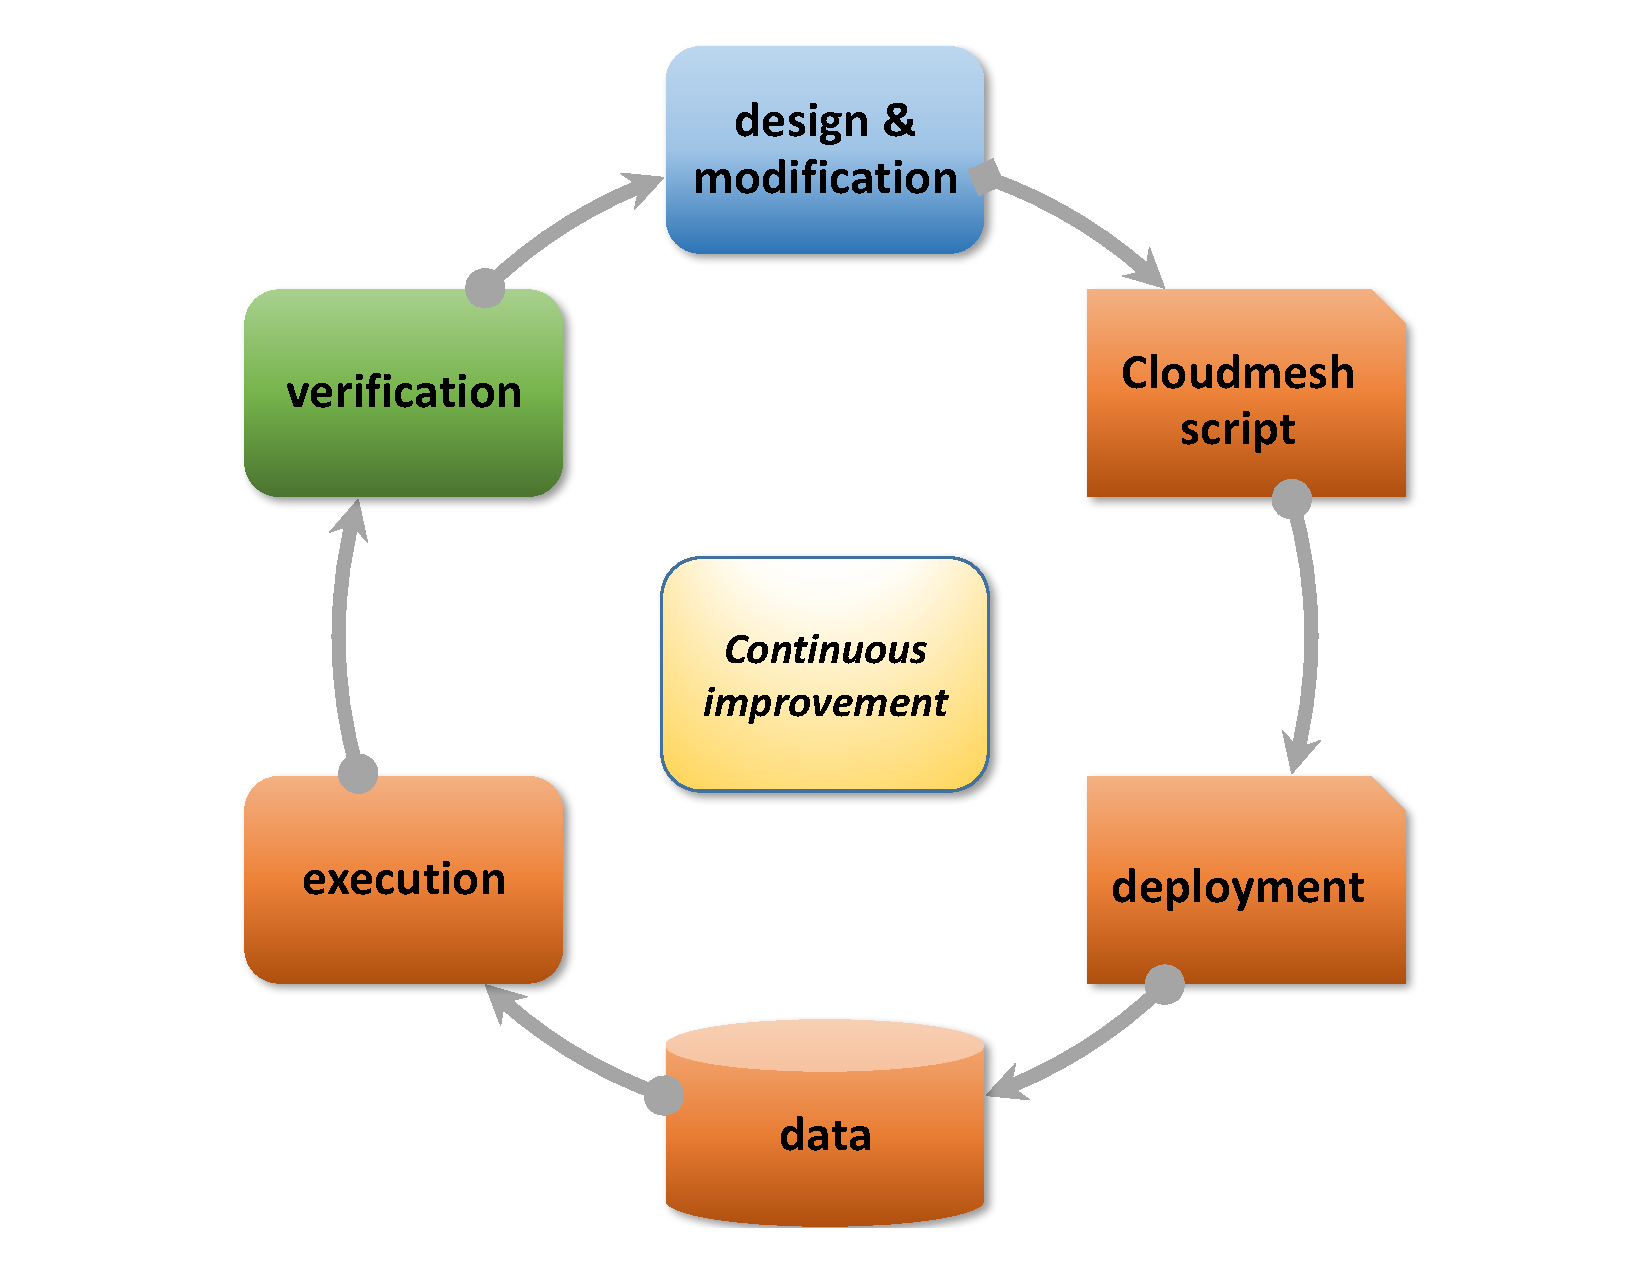
\includegraphics[width=1.0\columnwidth]{images/nist-devops-1.pdf}
  \caption{Continuous improvement while using cloudmesh interactively.}
  \label{F:NIST-arch}
%\end{figure}

\bigskip

%\begin{figure}[htb]
  \centering
      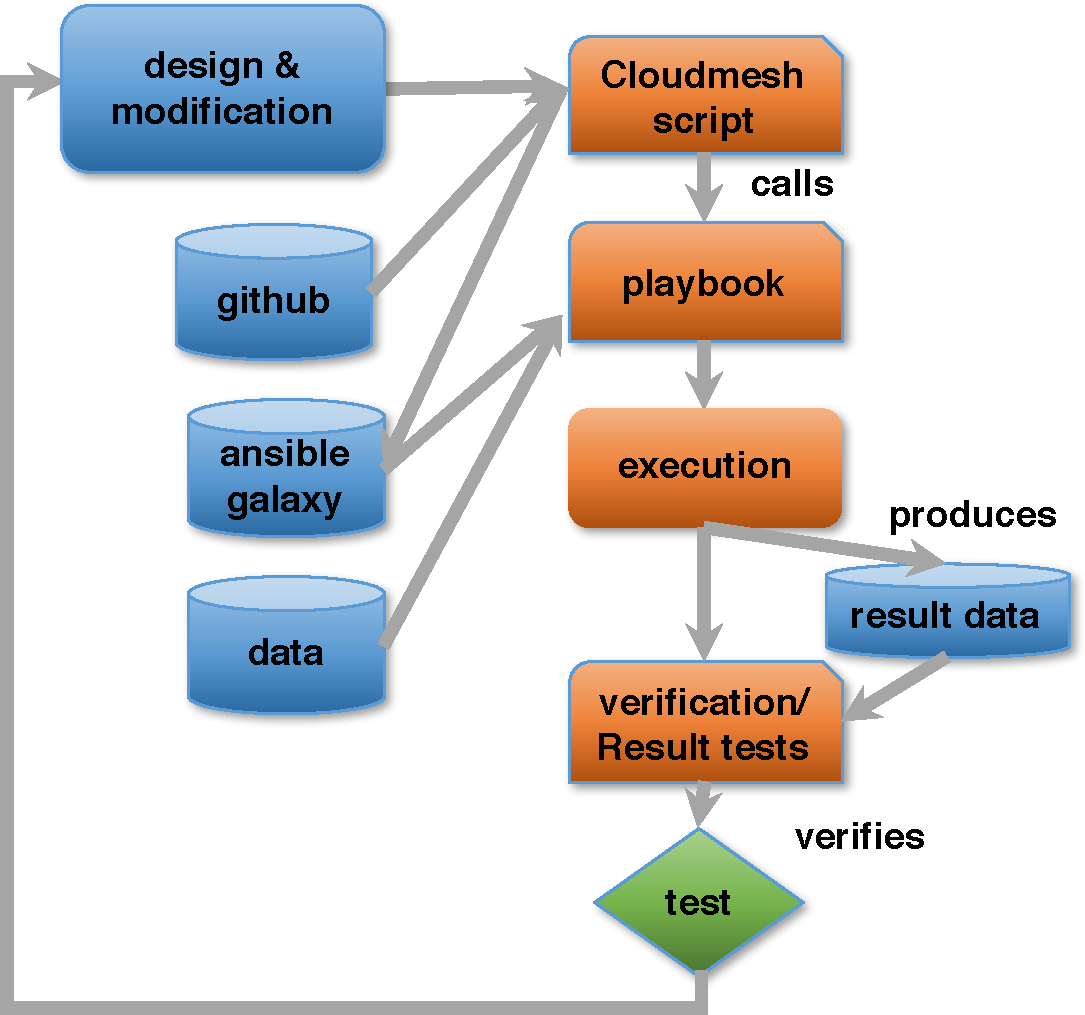
\includegraphics[width=0.8\columnwidth]{images/nist-devops-2.pdf}
  \caption{Interaction of the continuous improvement steps with
    various databases while using ansible deployment scripts.}
  \label{F:NIST-arch}
\end{figure}




\begin{description}

\item {\bf System Orchestrator} - provides high-level design dataflow
  between analytics tools and given datasets, computing system
  requirements, monitoring system resource and performance. At times
  the system orchestration is performed by the data scientist in an
  interactive manner. The system orchestrator is a service or
  component that acts in behalf of the data scientist, or another data
  science service that would require a particular configuration.

\item {\bf Data Provider} - provides abstraction of various types of 
data sources (such as raw data or data previously transformed by another system) 
and makes them available through different functional interfaces. This includes 
transfer analytics codes to data sources for effective analytic processing.


\item {\bf Big Data Application Provider} - provides analytics processing 
throughout the data lifecycle - acquisition, curation, analysis, visualization, 
and access - to meet requirements established by the System Orchestrator.


\item {\bf Big Data Framework Provider} - provides one or more instances 
of computing environment to support general Big Data tools, distributed file systems, 
and computing infrastructure - to meet requirements established by the Big Data 
Application Provider.


\item  {\bf Data Consumer} - provides interface to receive the value output 
from this NBD-RA ecosystem.


\item  {\bf Security and Privacy Fabric} - provides System Orchestrator 
the security and privacy interaction to the rest of the NBD-RA components to ensure 
protection of data and their content.


\item {\bf Management Fabric} - provides System Orchestrator the management 
interaction to the rest of the NBD-RA components with versatile system and software 
provisioning, resource and performance monitoring, while maintaining a high level 
of data quality and secure accessibility.

\end{description}




\section{Cloudmesh Client}
\label{S:cmclient}

The cloudmesh client toolkit is a lightweight client interface of
accessing heterogeneous clouds, clusters, and workstations right from
the users computer. The user can manage her own set of resources she
would like to utilize. Thus the user has the freedom to customize
their cyber infrastructure they use. Cloudmesh client includes an API,
a command-line client, and a command-line shell. It strives to abstract
backends to databases that are used to manage the workflow utilizing
the different infrastructure and also the services. Switching for
example to stage virtual machines from OpenStack clouds to amazon is
as simple as specifying the name of the cloud. Moreover, cloudmesh
client can be installed on Linux, MacOSX, and in future
Windows. Currently cloudmesh supports backends to SLURM, SSH,
OpenStack, AWS, and Azure. In the past we supported AWS and Azure.
Cloudmesh client allows to easily manage virtual machines, containers,
HPC tasks, through a convenient client and API. Hence cloudmesh is not
only a multi-cloud, but a multi-hpc environment that allows also to
use container technologies (under development). Additionally, we have
an example code on how to create a Web based portal with the help of
cloudmesh client.

\subsection{General Requirements and Goals}

Cloudmesh has from its inception followed the following general design
goals and requirements.

\begin{description}
\item [Technology agnostic.] An important aspect of cloudmesh is to
  offer access to useful services APIs and interfaces in a technology
  agnostic fashion. Thus it should be possible for example to switch
  easily between different IaaS providers. CM has excellently protected
  us during the changes of the OpenStack interfaces and libraries from
  the very first version of OpenStack. It also has allowed us to
  switch easily to different IaaS providers when it became clear that
  Eucalyptus was replaced by many with OpenStack.

\item[Easy to use.] Cloudmesh is supposed to make access of the
  complex workflow to integrate with IaaS and deploy on them new
  platforms and software stacks. This advanced feature is not only to
  be performed by expert IT personal or programmers, but in fact by
  data scientists which we found in practice have less experience in
  such areas. As we deal often with many compute nodes it is often
  insufficient to just provide a graphical user interface or portal, but
  we need to provide APIs, REST interfaces and especially command-line
  and shell access in an easy comprehensible fashion. 

\item[Expandable.] While working over the last years in the area it is
  obvious that the technology is rapidly evolving and new features
  need to be integrated, Thus it is important that cloudmesh is easy
  to expand and new features can be added while leveraging a core set
  of functionality and services.

\item[Documented.] Furthermore it is important that we provide from
  the start documentation to existing and new features and make it
  easy for the developers to contribute documented add ons, but also
  allow users to have access to documentation including examples. This
  will include easy to follow documented installation and configuration steps 
to guarantee successful deployment and use

\item[Repeatable and automated deployment.] When we install software
  stacks an a variety of platforms it is expected that that can easily
  be replicated and repeated automatically.

\item[Portable.] It is important to provide services in cross
  platforms compatible fashion. It ensures working, executable
  software deployment on multiple platforms. This includes not only
  the installation of the software, but the integration of external
  services and tools such as DevvOps or workflow frameworks that could
  support the general mission of a data scientist.

\item[Abstractions.] To address some of the design issues our
  requirements implicitly asks for the existence of a number of
  abstractions and interfaces that can be used to enable portable and
  crossplatform services and tools.

\end{description}

\subsection{Architecture Requirements and Goals}

In addition to the general requirements we set some specific
architectural requirements and goals that have been growing from
previous versions of cloudmesh and our earlier work in this area.

\begin{description}

\item{\bf Client based.} Cloudmesh client as the name indicates is a
  client based toolkit that is installed and run on the users
  computers. An add on component to use the client within a portal is
  available. Thus we distinguish the client that contains most of the
  functionality and the portal that can access the functionality
  through a locally maintaine Web portal. Important to note is that
  the user manages its own credentials and thus security and
  credential management is done directly on the users machine instead
  through a hosted Web portal. This increases the security as access
  to any credential is managed by the user and is not part of a
  credential management system.

\item{\bf REST.} Although Cloudmesh provides a client interface, it
will provide a REST interface to many of its services in order to
support service based deployments. The basic APIs developed for the
client can easily be reused to implement such interfaces.\footnote{we
  have demonstrated that cloudmesh APIs can be used to implement REST
  interfaces in a variety of frameworkks such as Flask, Django, and Cherypy}

\item{\bf Layered Architecture.} Cloudmesh client has a layered
architecture that allows easy development of new features. This also
allows contribution by the community while developing integrated and
smaller sub components. Figure A depicts the various layers. A
resource abstraction layer allows the integration of a multitude of
resources spanning HPC, Containers, and Cloud resources. (At this time
we focus on OpenStack and Slurm resources. We are working on
reintegrating resources such as Azure, AWS, Maui, Moab, and others
which we previously supported, as well as new resources such as
docker).

\item{\bf Management Framework.} Cloudmesh client contains a
management framework, and its components are depicted in Figure
B. cloudmesh allows easy management of virtual machines, containers,
and the data associated with them. We are currently developing a
choreography framework that leverages Ansible, chef, and heat. All of
the functionality is easily usable through a comand-shell that also
can be used from the command-line, and a Python API. IN future we will
be providing a REST API.

\item{\bf Database Agnostic.} Cloudmesh contains some state about the
resource and environment that a user may want to use. The information
is managed in an database abstraction that would allow storing the
data in a variety of databases such as SQL and MongoDB. At this time
we have chosen SQLite to be the default database as it does not
require any additional setup and is universally available on all
operating systems without change.

\item{\bf comand-shell and line.} Cloudmesh contains a comand-shell
allowing scripts to be developed and run. However we designed the
comand-shell in such a way that each command can also be called from
the command-line. Through the cloudmesh state machine the state
between comand-shell, command-client, and the portal is shared.

\item{\bf Cloudmesh Client Portal.} Previously, we distributed
cloudmesh with client, server, and a portal components in one
package. This however turned out to be to complex to be installed for
some of our less technically skilled user community. Thus we split up
the install into two independent packages. The cloudmesh client and
the cloudmesh portal. The portal provides some elementary features to
manage virtual machines and HPC jobs. At this time the portal is
considered to be alpha technology. Just as the client the portal is to
be run on the local user machine in oredr to allow increased security
by managing the credentials locally rather than on a server.

\item{\bf Cloudmesh Two Factor Authentication.} We have an
exploratory project in place that looks at the use of Yubikeys for
cloudmesh, client and cloudmesh portal.

\item{\bf Cloudmesh Comet.} We are actively developing the client
interface for SDSC’s comet supercomputer allowing bare metal
provisioning. The interface reuses cloudmesh components and
technologies while interfacing with the comet cloud REST
interface. The goal here is to manage virtual clusters.

\end{description}




\section{Cloudmesh Abstractions}

In this paper we will focus our attention to three important
abstractions that cloudmesh introduces: Cloudmesh Compute Experiments
(Section \ref{S:experiments}) , Cloudmesh Virtual Clusters (Section
\ref{S:vc}), Cloudmesh Stacks (Section \ref{S:stacks}).

\subsection{Compute Experiments} \label{S:experiments}

For many decades traditional supercomputing has provided large scale
resources to the research community. This is done in a shared
operating mode and enables researchers to utilize resources that they
otherwise would not have access to. Shared resources include
memory over a number of processors, shared disks, powerful processors
in speed and core numbers, fast interconnect. This has been applied to
many modeling applications but can naturally also be applied to big
data. In order to integrate such capabilities in a service oriented
fashion the Grid community has delivered prior to to e popularization
of cloudcomputing useful interfaces, API's, and toolkits. However for
research work that we supported with cloudmesh such interfaces and
efforts were to complex to use and we designed a simple model for
researchers that we worked with. This interface includes the abstract
concept of a ``job'' that is submitted to a queuing system and uses a
particular data set. The experiments in our case are repeated multiple
times and each run creates its own output directory.

Hence we have created a simple submission interface that submits the
script to the cluster. The script will be copied prior to execution
into the home directory on the remote machine. If a directory is
specified it will be copied into that dir.  The name of the output
directory is either specified in the script itself, or if not the
default naming scheme of cloudmesh is used using and the output
directory name is appended with an increasing index. To run such a
script we can on our client simply say
 
\begin{verbatim}
    cm hpc run SCRIPT
\end{verbatim}

Some more details about out improved interfaces are given in
Figure~\ref{T:rest}.

\begin{table*}[htb]
\caption{Selected Service Description}\label{T:rest}
\bigskip
\begin{center}
\begin{small}
\begin{tabular}{|l|l|l|}
\hline
\blue \textbf{Resource} & \blue \textbf{REST Method} & \blue \textbf{Description}\tabularnewline

%%%%%%%%%%%%%%%%%%%%%%%%%%%%%%%%%%%%%%%%%%%%%%%%%%%%%%%%%%%%%%%% Virtual cluster
\hline \multicolumn{3}{|l|}{\grey\bf Virtual Cluster: /cluster} \tabularnewline \hline
/                       & GET      & List available clusters \tabularnewline \hline
/                       & POST     & Launch a cluster on the provider \tabularnewline \hline
/                       & DELETE   & Delete all available clusters \tabularnewline \hline
/:id                    & DELETE   & Delete and destroy a cluster \tabularnewline \hline
/:id                    & GET      & View the status of a cluster (nodes, node type, etc) \tabularnewline \hline
/:id/property/:property & GET, PUT & Get/set a property (provider, name, description) of the cluster \tabularnewline \hline
/:id/inventory/:format  & GET      & Obtain an inventory of the cluster \tabularnewline \hline

%%%%%%%%%%%%%%%%%%%%%%%%%%%%%%%%%%%%%%%%%%%%%%%%%%%%%%%%%%%%%%%% Composition
\hline \multicolumn{3}{|l|}{\grey\bf Stack Composition: /stack} \tabularnewline \hline
/                               & GET      & List available compositions \tabularnewline \hline
/                               & POST     & Create a new composition \tabularnewline \hline
/:id                            & GET      & Show information about the composition \tabularnewline \hline
/:id                            & DELETE   & Delete a composition \tabularnewline \hline
/:id/name                       & GET, PUT & Get/set the name of the composition \tabularnewline \hline
/:id/add?deployer=:?\&source=:? & POST     & Add a layer to the composition \tabularnewline \hline
/:id/layer                      & GET      & List layers of the composition \tabularnewline \hline
/:id/layer/:id                  & DELETE   & Delete the layer of the composition \tabularnewline \hline

%%%%%%%%%%%%%%%%%%%%%%%%%%%%%%%%%%%%%%%%%%%%%%%%%%%%%%%%%%%%%%%% Stack Deployment
\hline \multicolumn{3}{|l|}{\grey\bf Stack Deployment: /stack} \tabularnewline \hline
/                    & GET  & List the available stacks with discription \tabularnewline \hline
/:id/deploy/:cluster & POST & Deploy a stack onto a cluster \tabularnewline \hline
/:id/status          & GET  & Get current status \tabularnewline \hline

 %%%%%%%%%%%%%%%%%%%%%%%%%%%%%%%%%%%%%%%%%%%%%%%%%%%%%%%%%%%%%%%% Batch
\hline \multicolumn{3}{|l|}{\grey\bf Batch Experiments: /hpc} \tabularnewline \hline
/                          & GET    & List all jobs started with the run command \tabularnewline \hline
/:id                       & DELETE & Deletes the experiment with the given id \tabularnewline \hline
/run?script=:?\&cluster=:? & POST   & Submits an experiment to the named cluster \tabularnewline \hline
/:id/status                & GET    & Returns the status of the job started with the run command \tabularnewline \hline

%%%%%%%%%%%%%%%%%%%%%%%%%%%%%%%%%%%%%%%%%%%%%%%%%%%%%%%%%%%%%%%% 

\end{tabular}
\end{small}
\end{center}
\end{table*}




\subsection{Cloudmesh Virtual Clusters} \label{S:vc}

Traditional HPC provided clusters to the community while  the clusters
are managed by professional staff and have mostly rigid software
stack targeting a broad community. Integration specialized software
stack and accessing the newest development based software is often
difficult or impossible to manage for a large number of
communities. Thus we see the following advantages and disadvantages:

\begin{description}

\item[Advantages:] provides well defined environment to the community,
  provides often optimized services for this particular system or the
  community it serves, allows sharing of resources through queuing
  system

\item[Disadvantages:] Different communities, groups or projects may
  have different requirements that are not met by the software stack,
  software stack often not state-of-the art, but tuned for
  reliability, experimentation with new software and methodologies in
  such an environment is difficult, queuing system may not provide
  enough interactivity

\end{description}

 Hence we are in the need of a mechanism to provide
clusters in a more manageable form. With the advent of virtualization
technologies, this can be achieved while users are provided with
virtual clusters hosted on cloud infrastructure using virtual machines,
or container virtualization software. This provides us with the
following advantages and disadvantages:

\begin{description}

\item[Advantages:] user stack provide a a more flexible and
  state-of-the-art environment; support different interaction modes
  with instantaneous access without wait time; support the use of
  heterogeneous platforms to allow increase in availability as well as
  features; and support the easy management of such an environment

\item[Disadvantages:] the user needs to manage the stacks themselves; a
  steep learning curve is needed to achieve this; the environment are
  feature rich and are difficult to manage

\end{description}

Naturally, cloudmesh is targeting to ease the disadvantages laid out.

\subsection{Groups} \label{S:groups}

One of the essential abs



\begin{table*}[htb]
\caption{Additional abstractions}\label{T:group}
\bigskip
\begin{center}
\begin{small}
\begin{tabular}{|l|l|l|}
\hline
\blue \textbf{Resource} & \blue \textbf{REST Method} & \blue \textbf{Description}\tabularnewline

 %%%%%%%%%%%%%%%%%%%%%%%%%%%%%%%%%%%%%%%%%%%%%%%%%%%%%%%%%%%%%%%% Additional abstractions
\hline \multicolumn{3}{|l|}{\grey\bf Groups: /group} \tabularnewline \hline
/                   & GET    & List all groups \tabularnewline \hline
/:id                & GET    & Returns the status of elements in the group \tabularnewline \hline
/:id                & DELETE & Deletes the group with the given id \tabularnewline \hline
/:id/member         & POST   & Add a new member to the group \tabularnewline \hline
/:id/member         & GET    & List the members of a group  \tabularnewline \hline
/:id/member/:member & PATCH  & Update a member from the group in the group \tabularnewline \hline
/:id/member/:member & DELETE & Deletes elements in the group \tabularnewline \hline

\end{tabular}
\end{small}
\end{center}
\end{table*}

\subsection{Virtual Clusters}

Definition: A set of compute, storage and network services that
interact with each other to serve an application or community for a
specific amount of time to support one or more experiments. A virtual
cluster is managed by the community or application user. They are
typically built on top of HPC, Grids, Clouds, and Containers. The
virtual cluster is managed by the user.

Contrasting Grids: targeted towards the support of a virtual
organization introducing high overheads on the deployment and
management of such infrastructure. Grids are a natural expansion of
traditional supercomputer centers that are managed by professional
staff. Contrasting Cloud IaaS: offer typically low level IaaS services
allowing users to combine them. They are a valuable building block for
virtual clusters. Clouds are managed by professional staff.

Contrasting Cloud PaaS: offer enhanced services to users targeting a
particular platform. They are offered by professional staff.

Contrasting Containers: offer an abstraction to share the existing hardware and OS while using containers making the it not necessary to us OS virtualization, thus saving space. Containers provide very useful enhancements for creating virtual clusters through add ons such as Kubernetes and Docker Swarm.



\subsection{Cloudmesh Access and Management of virtual clusters}
Cloudmesh is an API, command line tool, and command shell allowing the easy utilization of HPC, Clouds, Containers through machine abstractions
Switching between alternative services can be achieved by updating a
single variable.

Demonstrated usages of
Comet                                                                                           (HPC integrated Cloud)
FutureSystems, Chameleon, CloudLab, Bridges, Jetstream, …  (National Openstack Clouds)
Cybera (CA), Karslruhe Openstack Cloud (KIT, Germany), …     (International)
EC2, AWS, Azure                                                                          (Commercial Non Openstack)
Devstack, Trystack, Virtualbox                                                       (Desktop Clouds)
A user could use all of them

\subsection{Cloudmesh and Comet Cloud Virtual Cluster}
Comet is a NSF sponsored super computer offered by SDSC to the community. It operates in two modes: HPC and virtual clusters
Comet virtual clusters are low level and offer the HPC administrator the view of a cluster as if it were hardware. This is achieved via virtualization and low level exposure of network services. The administrator has full control over the cluster.
This is achieved by the integration of virtualization and SRIOV within Rocks. Thus the same cluster can not only be used in virtualized mode, but also in HPC mode
Comet users can therefore use HPC and virtualized clusters on the same hardware. Virtual clusters are treated as a special kind of compute job
Based on our long experience in this field we have delivered to SDSC an extension to cloudmesh that allows the creation and management of virtual clusters within comet
We can today use more than Comet
Accessing Virtual Clusters
REST API
Command line interface
Command shell for scripting
Console Access
Web Page

\begin{verbatim}
Simple commands allow easy management
cm comet cluster  ID
Show the cluster details
cm comet power on ID vm-ID -[0-3] --walltime=6h
Power 3 nodes on for 6 hours
cm comet image attach image.iso ID vm-ID-0
Attach an image
cm comet boot ID vm-ID-0
Boot node 0
cm comet console vc4
Console 

Switching infrastructure in cloudmesh is easy
cm var cloud=jetstream / bridges / aws / …
cm default cloud=$cloud
cm boot
\end{verbatim}

\subsection{Cloudmesh Launcher abstraction}
Important is that cloudmesh introduces an abstraction for creating virtual clusters that we call “launcher”. A launch specifies the creation of a virtual cluster. Such a launch can use
Ansible
Chef, …
Openstack Heat
Ssh
Make
Pegasus (Grids)
Hence a variety of different launch platforms can be integrated into cloudmesh and work from different community contributions can be supported.

Building virtual clusters is easy
cm launcher cluster -n 10
Gives a virtual cluster with 10 nodes and allows the user to login between each node


cm launcher hadoop -n 10 --cloud=rackspace
Finds the playbook for creating a hadoop cluster and launches it on a cloud called rackspace



Building enhance virtual clusters is easy
Virtual cluster for face detection
cm launcher facedetection -n 10 --cloud=rackspace
Finds the playbook for creating a virtual cluster and launches the deployment for the face detection project.
Cloudmesh will look in the git repository to locate the ansible scripts and execute them


Cloudmesh Launcher Portal (in development)
       Specific Launch                                    List of Launchers





Automatically generates Graphical representation of input parameters                                  


\subsection{Cloudmesh Stack}
\label{S:stacks}

The cloudmesh stack command tackles the problem of reproducibly
deploying software stacks and packages on virtual clusters.

A ``stack'' is a way to modify a collection of accessible nodes in
order to bring them to a desired state. This execution unit should be
able to use multiple different deployment technologies: eg Ansible,
Chef, Puppet, NixOS, shell scripts, etc. These deployment units are
then composed (a ``stack composition'') into layers to form a new
deployment unit that can be used as a layer within a different
composition. See Figure~\ref{F:stack-composition} for an illustration.


\begin{figure}
\centering
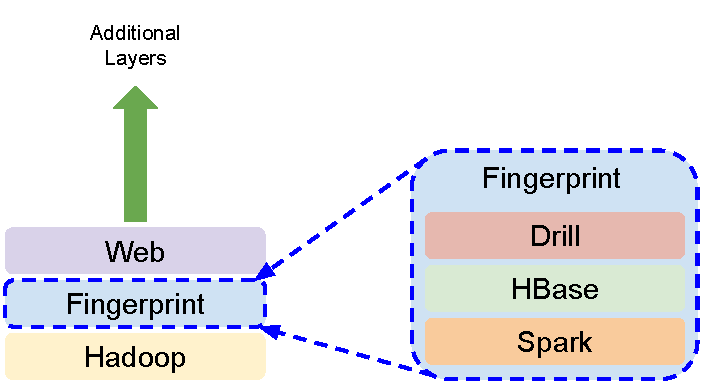
\includegraphics[width=1\columnwidth]{images/cloudmesh-stack-composition.pdf}
\caption{This shows how stacks may be composed. The
  \texttt{Fingerprint} stack is a composition of the Apache
  \texttt{Drill}, \texttt{HBase}, and \texttt{Spark}
  stacks. \texttt{Fingerprint} is then included as a layer withing
  another composition built upon \texttt{Hadoop} and extended with the
  \texttt{Web} layers. The \texttt{Web} layer itself may be composed
  of other layers.
  \label{F:stack-composition}}
\end{figure}
\TODO{Gregor,
  \href{https://docs.google.com/drawings/d/15zxYCF9cOUpd_X96HwtNW6ftJSGVhOnMSsObT1gUoDw/edit}{link
    to figure source}}


The stack command deploys and configures a user-defined subset of the
available modules while leveraging existing deployment technologies.

Cloudmesh provides a number of predefined modules such as Apache Spark
and Apache Drill that can be reused and customized on the virtual
cluster. This results in a minimization of work on the user as we as
the cloudmesh team as a number of existing deployments that are
available on the internet can be leveraged. However cloudmesh provides
a valuable add on as it demonstrates and showcases the use of some of
these deployments while also vetting and improving them.


The stack command was initially developed to aid students and
researchers in completing data analytics projects.  They were faced
with exploring various technologies and would get stuck during the
installation and configuration phase, unable to progress due to the
complexity involved in managing it. While making cloudmesh stack
available and targeting often used deployment stacks we wer able to
assist these groups significantly.  The cloudmesh stack command has
been initially called {\em launcher} but has been renamed to {\em
  stack} to make it more clear that it is more than starting a
program. It reuses technologies defined in \TODO{\cite{}
  https://github.com/futuresystems/big-data-stack}. The first step is
to define a virtul cluster with the cluster command, than we execute
one or more stack commands on the inventory that is returned by the
cluster command.

\begin{Verbatim}[fontfamily=helvetica]
$ cm default cloud=$CLOUDNAME
$ cm cluster create --count 4
$ cm stack create
$ cm stack layer hadoop
$ cm stack layer spark --deployer chef
$ cm stack deploy
$ cm stack deploy drill
\end{Verbatim}


\subsubsection{Stack Composition} \label{S:composition}
\TODO{Badi}


\subsubsection{Language for Interpreted Stack Programming} \label{S:stack-lisp}
\TODO{Badi, title}


\subsubsection{Integration of Deployment Tools}

various deployment tools and approaches

\begin{description}
\item[Scripts]
\item[Programs]
\item[OpenStack Heat]
\item[Ansible]
\item[Chef]
\item[Puppet]
\item[Salt]
\item[Vagrant]
\end{description}

\subsection{Cloudmesh stack}

\begin{Verbatim}[fontfamily=helvetica]
stack check [--stack=bds]
stack init [--no-activate] [--branch=master] [--user=$USER] 
               [--name=<project>] <ip>...
stack list [--sort=<field=date>] [--list=<field,...=all>] [--json]
stack project [<name>]
stack deploy [<play>...] [--define=<define>...]

Options:
   --format=FORMAT  the output format [default: table]
   --cloud=CLOUD    the cloud name
\end{Verbatim}

\subsection{Create a hadoop cluster}

\begin{Verbatim}[fontfamily=helvetica]
$ cm hadoop start --user cc --name=cluster_1
$ cm delete --name=cluster_1 --all  
\end{Verbatim}


\section{BDS}

\subsection{Deployment}

Big Data Software Stack is built with various software packages from different layers (and it’s increasing), therefore accomplishing these multiple software deployment is challenging



\section{Big Data Stack (BDS)}

BDS is a collection of playbooks for deploying the tools of big data analytics, given a set of accessible IP addresses. It allows the user to select a subset of the available tools to deploy in order to customize their virtual cluster.

Example: to setup a stack with Hadoop, Spark, and Hive:
$ ansible-playbook play-hadoop.yml addons/spark.yml addons/hive.yml
Example: to setup a stack with Hadoop, HBase, and Drill:
$ ansible-playbook play-hadoop.yml addons/hbase.yml addons/drill.yml
It is provided online at https://github.com/futuresystems/big-data-stack

\begin{description}

\item[Roles:]
Drill,
Ganglia,
Hadoop,
Hbase,
Hive,
Java,
Limits,
Maven,
Mysql,
Nagios,
Pig,
Spark,
Supervisord,
Zookeeper

\item[Playbooks:]
Hadoop
Hbase
Pig
Spark
Drill
Hive
\end{description}

\subsection{Towards Cloudmesh}
BDS is ideally suited to be included in cloudmesh as one of its deployment management tools. Cloudmesh adds features to easily access infrastructure.
  … more in the next another section we present later

Examples
Face Detection Example
Example 1: Face Detection Lifecycle
\begin{Verbatim}
[masters]
10.0.0.1
10.0.0.2
10.0.0.3
[workers]
10.0.0.4
10.0.0.5
10.0.0.6
Example 1: Face Detection Lifecycle on AWS
[masters]
10.0.0.1
10.0.0.2
10.0.0.3
[workers]
10.0.0.4
10.0.0.5
10.0.0.6
u'tag_masters_True': [u'52.23.213.103', u'54.196.41.145',u'54.209.137.235'],
u'tag_workers_True': [u'52.23.213.104', u'54.196.41.146',u'54.209.137.237'], ...
\end{Verbatim}

Example 1: Face Detection Screenshot Running EC2 provisioning playbook
on command line:

\begin{Verbatim}
$ ansible-playbook boot-ec2-with-vpc.yml -i ec2.py
\end{Verbatim}

\subsection{Conclusion}
Ansible + Cloudmesh
Will enable re-usable specification of Big Data Stack applications in 87 use cases and 62 unique roles from which NIST has 27
BDS status
From this a total part of BDS are vetted (the most fundamental ones): 
14 Roles  (about 50% done of NIST roles)
6   Playbooks

\subsection{Cloudmesh Status}
We can replicate on different infrastructures including AWS, Azure, Openstack, Comet …
We need to complete the launcher and integration of the BDS into the launcher





%%%%%%%%%%%%%%%%%%%%%%%%%%%%%%%%%%%%%%%%%%%%%%%%%%%%%%%%
\section{Big Data Use Cases}\label{S:usecases}

The NIST Big Data Working group has identified 51 benchmarking examples for Big Data\cite{??} spanning application areas such as:

\begin{description}

\item[Government Operation:] National Archives and Records
  Administration, Census Bureau

\item[Commercial:] Finance in Cloud, Cloud Backup, Mendeley
  (Citations), Netflix, Web Search, Digital Materials, Cargo shipping
  (as in UPS)

\item[Defense:] Sensors, Image surveillance, Situation Assessment
  Healthcare

\item[Life Sciences:] Medical records, Graph and Probabilistic
  analysis, Pathology, Bioimaging, Genomics, Epidemiology, People
  Activity models, BiodiversityDeep Learning and Social Media: Driving
  Car, Geolocate images/cameras, Twitter, Crowd Sourcing, Network
  Science, NIST benchmark datasets

\item[The Ecosystem for Research:] Metadata, Collaboration, Language
  Translation, Light source experiments

\item[Astronomy and Physics:] Sky Surveys compared to simulation,
  Large Hadron Collider at CERN, Belle Accelerator II in JapanEarth,

\item[Environmental and Polar Science:] Radar Scattering in
  Atmosphere, Earthquake, Ocean, Earth Observation, Ice sheet Radar
  scattering, Earth radar mapping, Climate simulation datasets,
  Atmospheric turbulence identification, Subsurface Biogeochemistry
  (microbes to watersheds), AmeriFlux and FLUXNET gas sensors

\item[Energy:] Smart grid

\end{description}

In addition we have 81 student projects from classes taught at Indiana University on the topic of Big Data. 
From these examples we have examined on six of the NIST uses case projects to identify the technologies used as shown in Table~\ref{T:usecases}.

\begin{table}[htb]
  \bigskip
  \setlength\tabcolsep{2pt}
  \caption{
    Technology used in a subset of usecases. A \OK~indicates that the technology is used in the given project. See Table~\ref{T:usecase2} for details on a specific project. The final row aggregates \OK~across projects.}
  \label{T:usecases}
  \bigskip
  \begin{small}
    \begin{center}
      \resizebox{\columnwidth}{!}{
        \begin{tabular}{|c|*{23}c|}
          \hline

          ID & \rot{Hadoop} & \rot{Mesos} & \rot{Spark} & \rot{Storm} & \rot{Pig} & \rot{Hive} & \rot{Drill} & \rot{HBase} 
             & \rot{Mysql} & \rot{MongoDB} & \rot{Mahout} & \rot{D3 and Tableau} & \rot{nltk} & \rot{MLlib} 
             & \rot{Lucene/Solr} & \rot{OpenCV} & \rot{Python} & \rot{Java} & \rot{Ganglia} & \rot{Nagios} & \rot{zookeeper} & \rot{AlchemyAPI}
             & \rot{R} \\ \hline

          % ID  & Hadoop & Mesos & Spark & Storm & Pig & Hive & Drill & HBase & msql & mongo & mht & D3/T & nltt & mllib & lu/slr & OCV & Py  & Java & Gngla & Ngs & ZK  & AlchemyAPI & R   
          N$_1$ & \OK    &       & \OK   &       &     & \OK  & \OK   & \OK   & \OK  &       &     &      &      &       &        &     &     & \OK  & \OK   & \OK & \OK &            &     \\ \hline
          N$_2$ &        & \OK   & \OK   &       &     &      &       &       &      &       &     &      &      &       &        & \OK & \OK &      &       &     & \OK &            &     \\ \hline
          N$_3$ &        &       &       & \OK   &     &      &       & \OK   &      & \OK   &     & \OK  & \OK  &       &        &     & \OK & \OK  &       &     & \OK & \OK        & \OK \\ \hline
          N$_4$ & \OK    &       & \OK   &       &     &      &       & \OK   &      &       & \OK & \OK  &      & \OK   & \OK    &     &     & \OK  &       &     & \OK &            &     \\ \hline
          N$_5$ & \OK    &       & \OK   &       &     &      &       &       &      &       & \OK & \OK  &      & \OK   &        &     &     & \OK  &       &     &     &            &     \\ \hline
          N$_6$ & \OK    &       & \OK   &       & \OK & \OK  &       & \OK   &      & \OK   & \OK & \OK  &      & \OK   & \OK    &     &     & \OK  &       &     & \OK &            &     \\ \hline
          count & 4      & 1     & 5     & 1     & 1   & 2    & 1     & 4     & 1    & 2     & 3   & 4    & 1    & 3     & 2      & 1   & 2   & 5    & 1     & 1   & 5   & 1          & 1   \\ \hline

        \end{tabular}
      }
    \end{center}
  \end{small}
\end{table}


\begin{table*}[htb]
  \caption{Dataset used in the various use cases.}
  \bigskip
  \label{T:usecase2}
  \begin{center}
    \begin{tabular}{|c|p{0.8\columnwidth}|p{0.8\columnwidth}|c|}

      \hline

      ID    & Use Case                                                                & Dataset                                                                      & Size (GB) \tabularnewline \hline
      N$_1$ & Fingerprint Matching                                                    & Special Database 14 - NIST Mated Fingerprint Card Pairs 2                    & 2.1       \tabularnewline \hline
      N$_2$ & NIST Human and Face Detection                                           & INRIA Person Dataset                                                         & 0.96      \tabularnewline \hline
      N$_3$ & NIST Twitter Analysis                                                   & Twitter                                                                      & -         \tabularnewline \hline
      N$_4$ & NIST Analytics for Healtcare Data / Health Informatics                  & Medicare Part-B in 2014 from Center for Medicare and Medicaid Services (CMS) & 0.1       \tabularnewline \hline
      N$_5$ & NIST Spatial Big Data/Spatial Statistics/Geographic Information Systems & Uber                                                                         & 0.2       \tabularnewline \hline
      N$_6$ & NIST Data Warehousing and Data Mining                                   & United States 2010 Census data                                               & -         \tabularnewline \hline

    \end{tabular}
  \end{center}
\end{table*}


Deployment of a single technology may result in development of several ansible roles comprising dependencies.
The implementation of the Fingerprint usecases (N$_1$) Ansible playbook uses 19 such roles that may be reused in other projects and Face Detection (N$_2$) uses five.
Furthermore, The remaining four NIST use cases N$_4$ - N$_6$ (Twitter analysis, Healthcare, Spatial data, Data Wharehousing) may contribute an addition 27 roles.

In summary, we have looked at 6 projects from the 51 NIST use cases to identify 51 Ansible roles.
Looking through 81 class projects over two semesters at Indiana University showed 62 roles, of which a subset were found to be repeatedly used across various projects.

% In addition we analyzed 36 projects from a big data class taught at
% Indiana University in Spring '16. Here we identified 41 roles in 45
% projects showcasing a wide divergent use case scenario.  A similar
% class thought in Fall '15 resulted in 62 roles while using 39
% datasets.




\subsection{Fingerprint Matching (N$_1$)}

Fingerprint recognition refers to the automated method for verifying a
match between two fingerprints and that is used to identify
individuals and verify their identity. Fingerprints are the most
widely used form of biometric used to identify individuals. The
automated fingerprint matching generally required the detection of
different fingerprint features (aggregate characteristics of ridges,
and minutia points) and then the use of fingerprint matching
algorithm, which can do both one-to- one and one-to- many matching
operations. Based on the number of matches a proximity score (distance
or similarity) can be calculated. Furthermore, NIST is providing via
the the NIST Fingerprint dataset a special database. The goal for this
usecase is the following: given a set of {\it probe} and {\it gallery}
images, compare the probe images to the gallery images, and report the
matching scores.  The dataset comprises 54,000 images and their
metadata.  It uses MINDTCT \cite{mindtct} preprocesses the images
to identify minutae of the prints automatically locating and recording
ridge ending and bifurcations in a fingerprint image; and BOZORTH3
\cite{garris2001user} to identify matches. Both are are part of the NIST
Biometric Image Software (NBIS) \cite{watson2007user}.

To execute this usecase we need to deploy an application to analyze
the dataset. It internally uses cloudmesh to deploy an the software
stack The implemented \cite{nist-fingerprint}
solution uses a software stack comprising of HDFS, YARN, Apache Spark,
Apache HBase, and Apache drill, Scaka, and the NBIS software. A Hadoop
cluster is deployed and YARN used to schedule Spark jobs that load the
images into HBase, process the images, and compute the matches. Apache
Drill, with the HBase plugin, can then be used to generate reports
with the NBIS tools\cite{watson2007user}. The results are stored in HBase and
Apache Drill \cite{??} is used to query the results.  The code
leverages tools and services is based on \cite{nist-bd-pwg}, while significantly
enhancing it with cloudmesh deployment strategies and services.

\cite{flanagan2010nist}
\TODO{Hyungro: create citation for this. http://www.nist.gov/itl/iad/ig/nbis.cfm}

\subsection{Face Detection (N$_2$)}

\TODO{Hyungro: define the references}

Human detection and face detection have been studied during the last
several years and models for them have improved along with Histograms
of Oriented Gradients (HOG) \cite{dalal2005histograms} for Human Detection. 



We use OpenCV \cite{bradski2000opencv}, a Computer Vision library including the
Support Vector Machine (SVM) classifier, and the Histogram of Oriented
Gradient (HOG) \cite{dalal2005histograms}object detector for pedestrian detection and
INRIA Person Dataset is one of popular samples for both training and
testing purposes. HOG with SVM model is used used as object detectors
and classifiers while the python libraries from OpenCV provide these
models for human detection.  The OpenCV Python code runs with Spark
Map function to perform distributed job processing on the Mesos
scheduler.

To enable this analysis we use cloudmesh to deployed Apache Spark on a
Mesos clusters and install the OpenCV software and its Python API. We
also update the python software stack. Then we to train and apply
detection models from OpenCV using Python API. We use the INRIA Person
Dataset \cite{dalal2005inria}. This dataset contains positive and negative images for
training and test purposes with annotation files for upright persons in each
image. 288 positive test images, 453 negative test images, 614 positive
training images and 1218 negative training images are included along with
normalized 64x128 pixel formats. The size of the dataset is 970MB.

Cloudmesh deploys and builds the clusters for batch-processing large
datasets, Internally cloudmesh uses for this ansible scripts to
support installation and configuration while leveraging available
cloud compute resources. We have for this example developed or are
reusing five ansible roles that we developed for other usecases::
Apache Spark \cite{ansible-role-spark}
Apache Mesos \cite{hindman2011mesos}, Apache Zookeeper
\cite{hunt2010zookeeper}, \TODO{Hyungro: make reference out of: Ansible Role
  for Mesos (with Zookeeper):
  https://github.com/VirtualClusters/ansible-role-mesos-by-mesosphere}
  OpenCV (with Python) \cite{ansible-role-opencv}



\cite{nist-facedetection}
\TODO{Hyungro: make reference out of: Ansible Main Play (Include Statement): https://github.com/futuresystems/pedestrian-and-face-detection}

\TODO{Hyungro: add also the original pointed and not just the ansible citation,
e.g. each should have to citations}



%%%%%%%%%%%%%%%%%%%%%%%%%%%%%%%%%%%%%%%%%%%%%%%%%%%%%%%%

\section{Conclusion}

\TODO{add conclusion}

\subsection{Future Works}

\TODO{discuss additional work}

\TODO{server less computing \cite{hil16}} 

\TODO{server less computing \cite{cloud3}} 
